\newpage
\section{Plots}
\label{sec:Plots}

Here is a section of common plots that were produced with the GeanePlots module. These plots were generated with the makeGEANEPlots.fcl file with version v7\_06\_01 for truthLRFit tracks. There is no plane number cut in these plots, but there is a truth energy cut of 3 MeV to cut out some poor events. The tracks these plots describe were generated starting with 7000 muons times 500 grid jobs, 3.5 M muons, with the mdc1.fcl file, resulting in approximately 140,000 tracks. All three trackers were included in the simulation, unnecessary geometry was omitted (such as calorimeters), the trajectory art records were not recorded, orphans were not tracked, and normal material was included. If checking out this documentations repository, then the analyzer root file is located in ``Images/MainPlots/gm2GEANE\_ana\_19831354\_1504040981.139.root''.

Branch and commit numbers used to generate these plots are listed below: \\

artg4 - feature/trackDevelop - ed5436 \\

gm2analyses - develop - b470cb7 \\

gm2dataproducts - feature/trackDevelop - 4fb1dc \\

gm2geom - feature/trackDevelop - c623aa9 \\

gm2ringsim - feature/trackDevelop - 9684d18 \\

gm2tracker - feature/trackDevelop - aa9239e \\

gm2util - feature/trackDevelop - 17b7856 \\

The sam-data-set names are ``nkinnaird\_documentation\_events\_mdc1\_reduced'' and \\
``nkinnaird\_documentation\_tracks\_truthLRFit'' for the events and tracks respectively.
Some more information including the locations of the sam-data-sets and root files are included in the directory: \\
``/pnfs/GM2/persistent/Tracking/nkinnaird/Documentation''

\begin{figure}
    \centering
    \begin{subfigure}[]{0.45\textwidth}
        \centering
        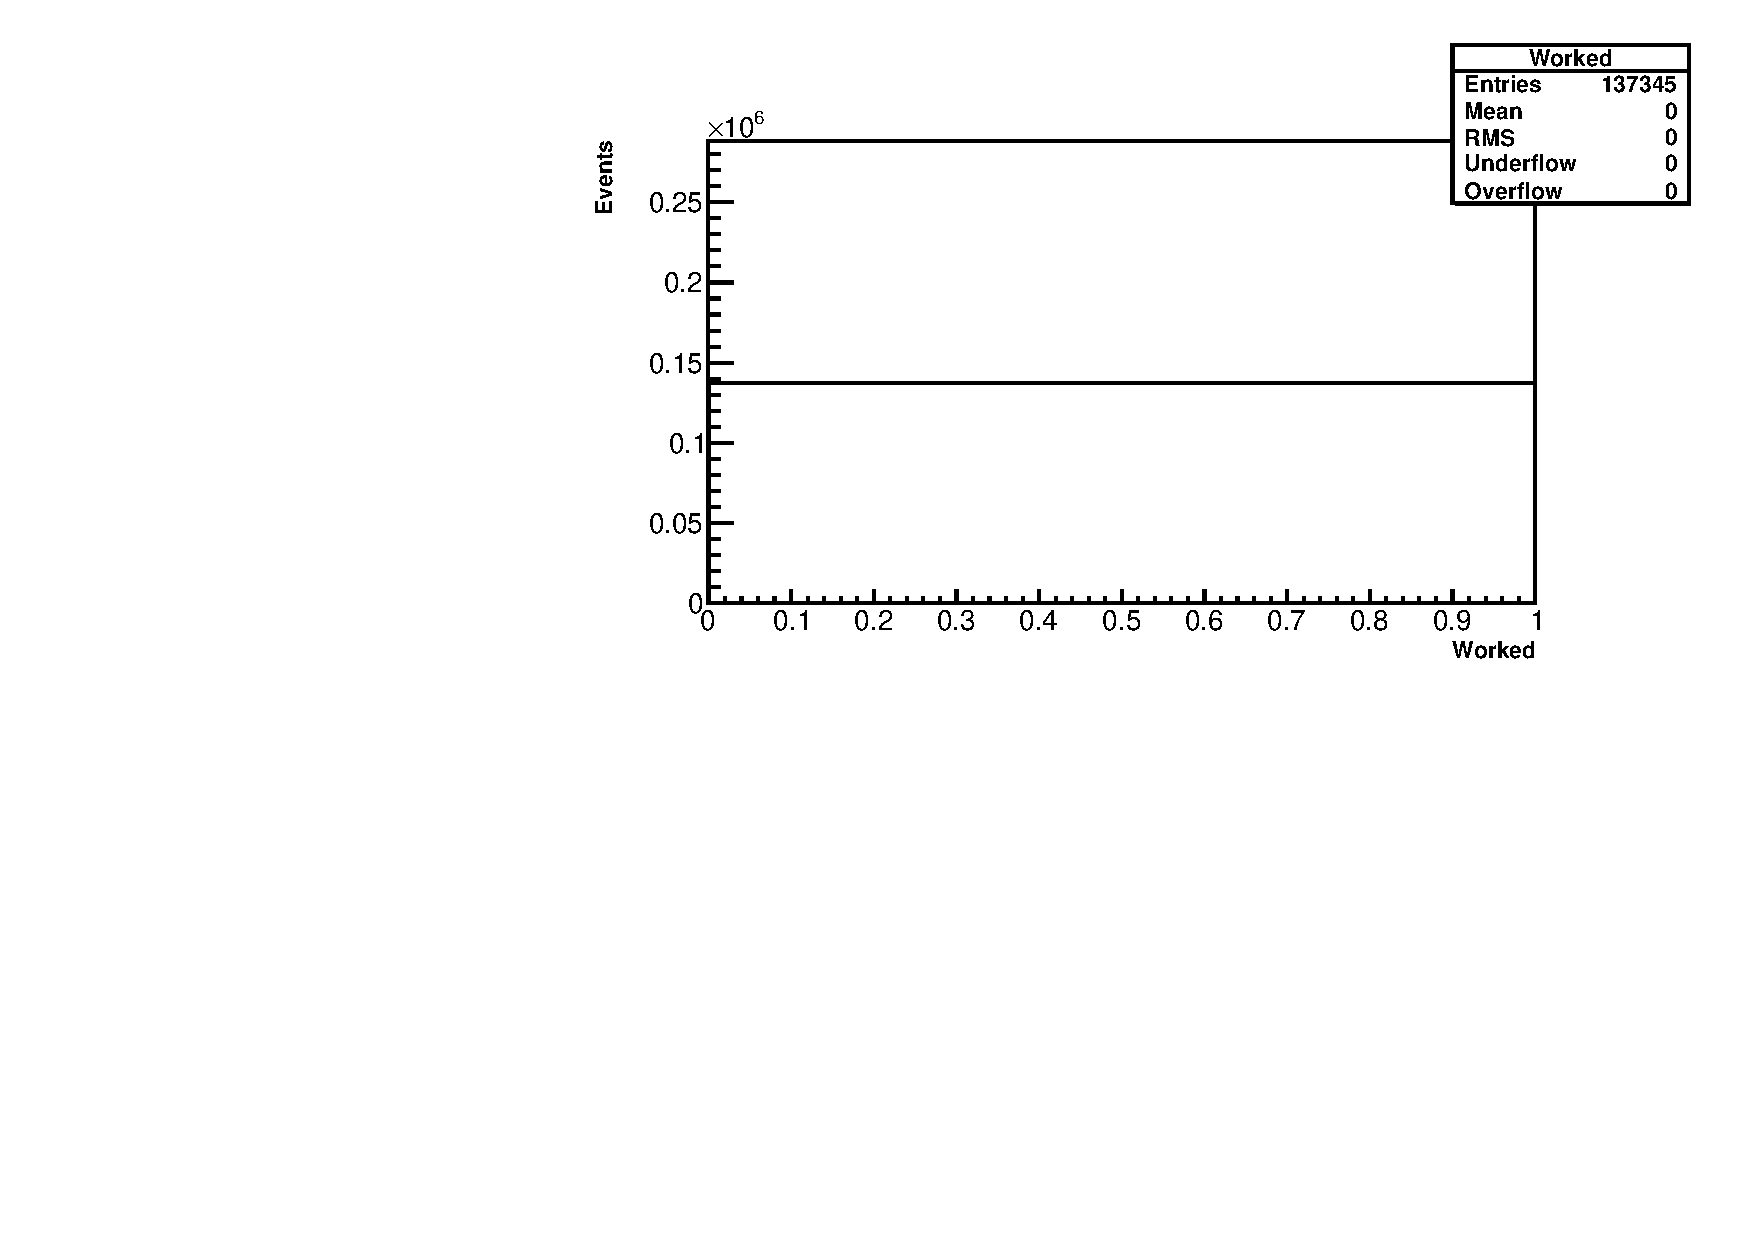
\includegraphics[width=1\textwidth]{WorkedEvents} 
        \caption{Generic}
        \label{fig:timing1}
    \end{subfigure}
    \hfill
    \begin{subfigure}[]{0.45\textwidth}
        \centering
        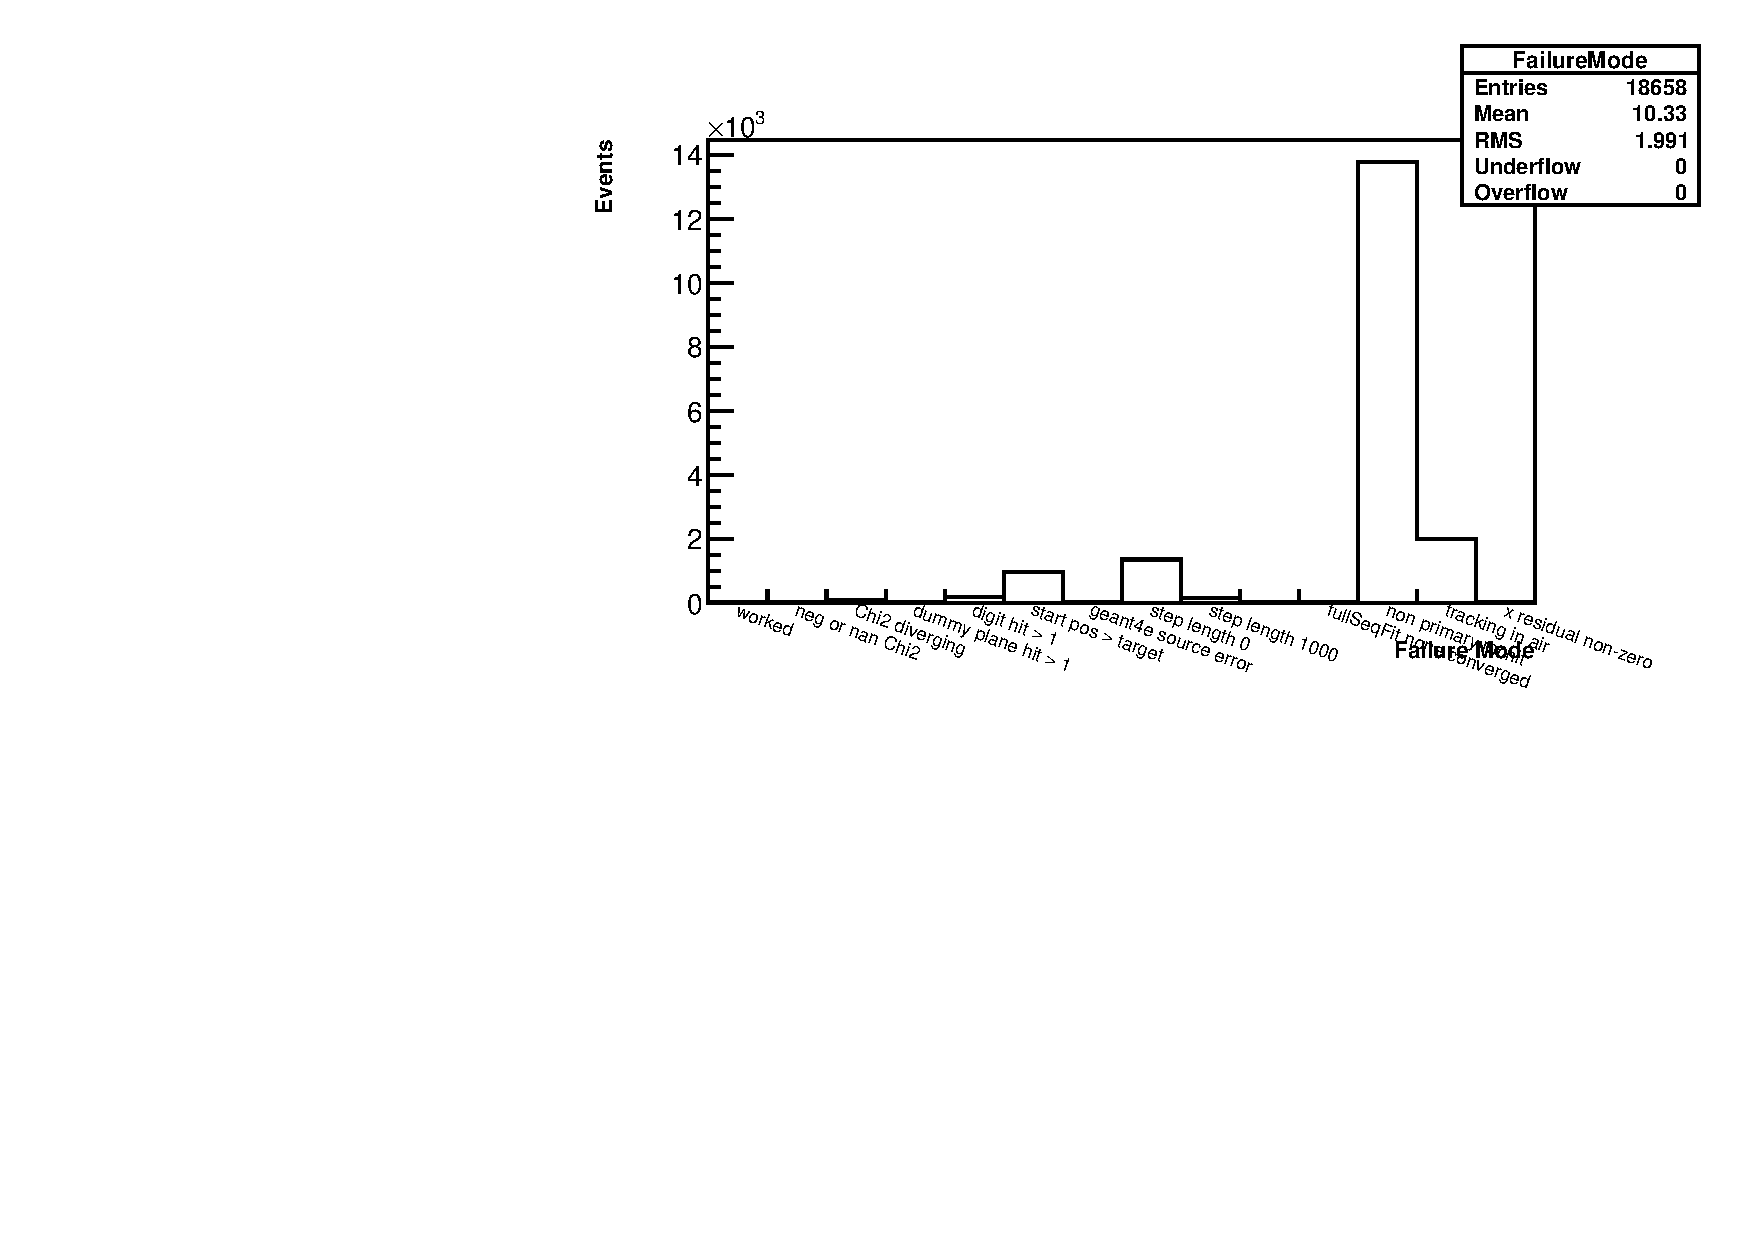
\includegraphics[width=1\textwidth]{FailedEventsUnzoomed} 
        \caption{Competitors}
        \label{fig:timing2}
    \end{subfigure}

    \vspace{1cm}
    \begin{subfigure}[]{0.45\textwidth}
        \centering
        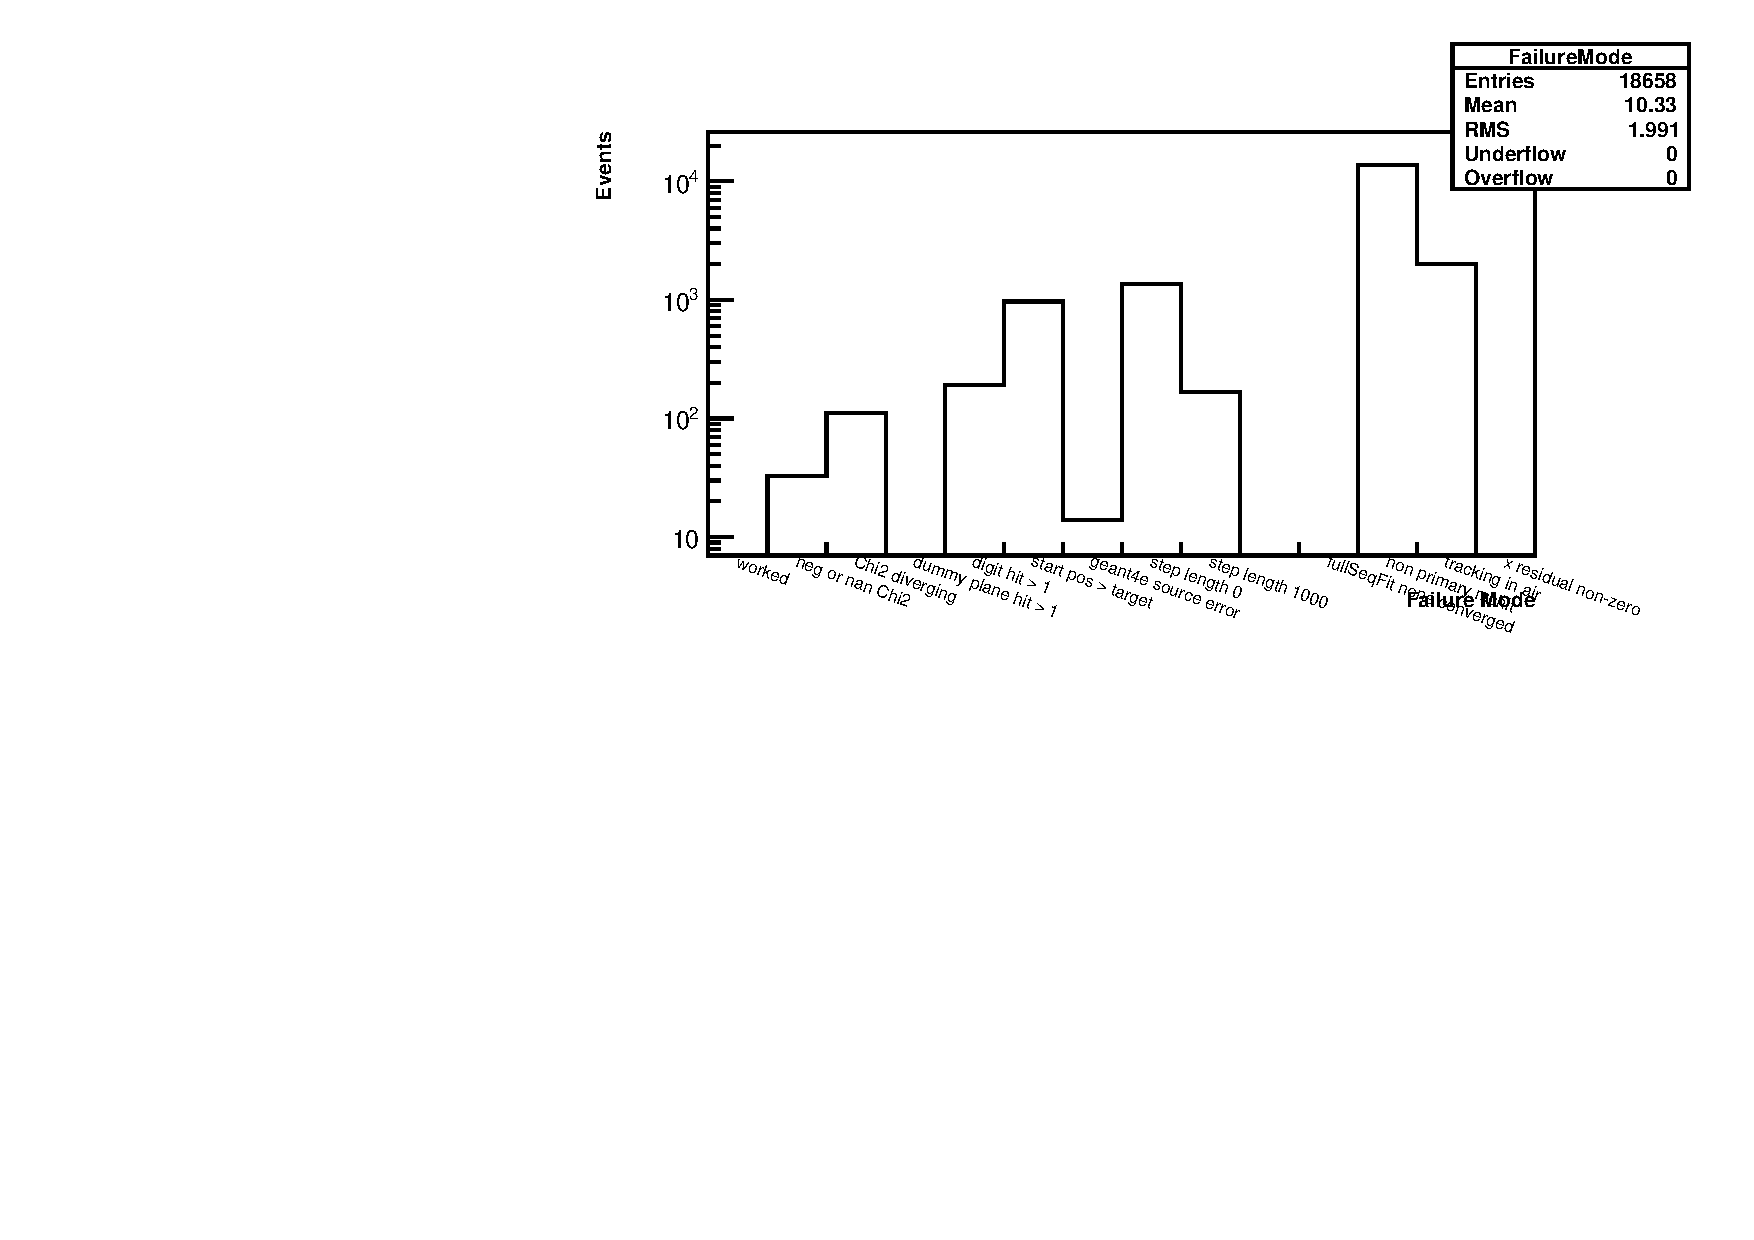
\includegraphics[width=1\textwidth]{FailedEventsLog} 
        \caption{Price regulation}
        \label{fig:timing3}
    \end{subfigure}
    \hfill
    \begin{subfigure}[]{0.45\textwidth}
        % just an empty subfigure to shift C below A
    \end{subfigure}
    \caption{Some general caption of all the figures. In (\subref{fig:timing1}) you can see a  green square....}
\end{figure}





















	% \begin{figure}[]
	% 	\caption{}
	% 	\centering
	% 	\includegraphics[width=0.3\textwidth]{title}
	% 	\label{fig:title}
	% \end{figure}
